% background.tex

\documentclass[main.tex]{subfiles}
\begin{document}
\chapter{Background}
\section{Additive Manufacturing}\label{sec:AM} %Section labeling for cross-referencing
\emph{Additive Manufacturing} (AM) technologies had their beginnings in the decade of the 1980s. During this time, various independently developed patents were filed across the globe describing a process that would construct an object by selectively adding layers of material -as opposed to removing excess matter or deforming the material to obtain the desired shape. This represents the core definition of AM: any technology where the final geometry of the manufactured object is obtained through controlled addition of material qualifies as an Additive Manufacturing technique \cite{Gibson2015}.

Advancements in the fields of computing, \emph{Computer Aided Design} (CAD), and controllers, among other technological developments, were necessary to translate the patents into working prototypes, with some eventually becoming the foundations of commercially successful companies -such as 3D Systems in 1986 and Stratasys in 1989 \cite{Gibson2015,3DSystems,Stratasys2017}. However, the basic process of AM has remained largely unchanged from its first iteration in the late 80s: First, a computer model of the object is made using CAD software and exported under the .\emph{stl} file format. Afterwards, the part geometry is stratified, or \textquotedblleft sliced\textquotedblright, and translated into machine instructions using a specialized software called \emph{slicing engine}. An AM machine then follows said instructions, commonly referred to as the \emph{toolpath}, to build the object in layers. Finally, the part is available to the user. Depending on either the requirements of the part, or the specifics of the AM technique used, some post-processing may be required \cite{Gibson2015}. A visual representation of the process is shown in Figure~\ref{fig:AM_flow}.

\begin{figure}[h]
	\center
	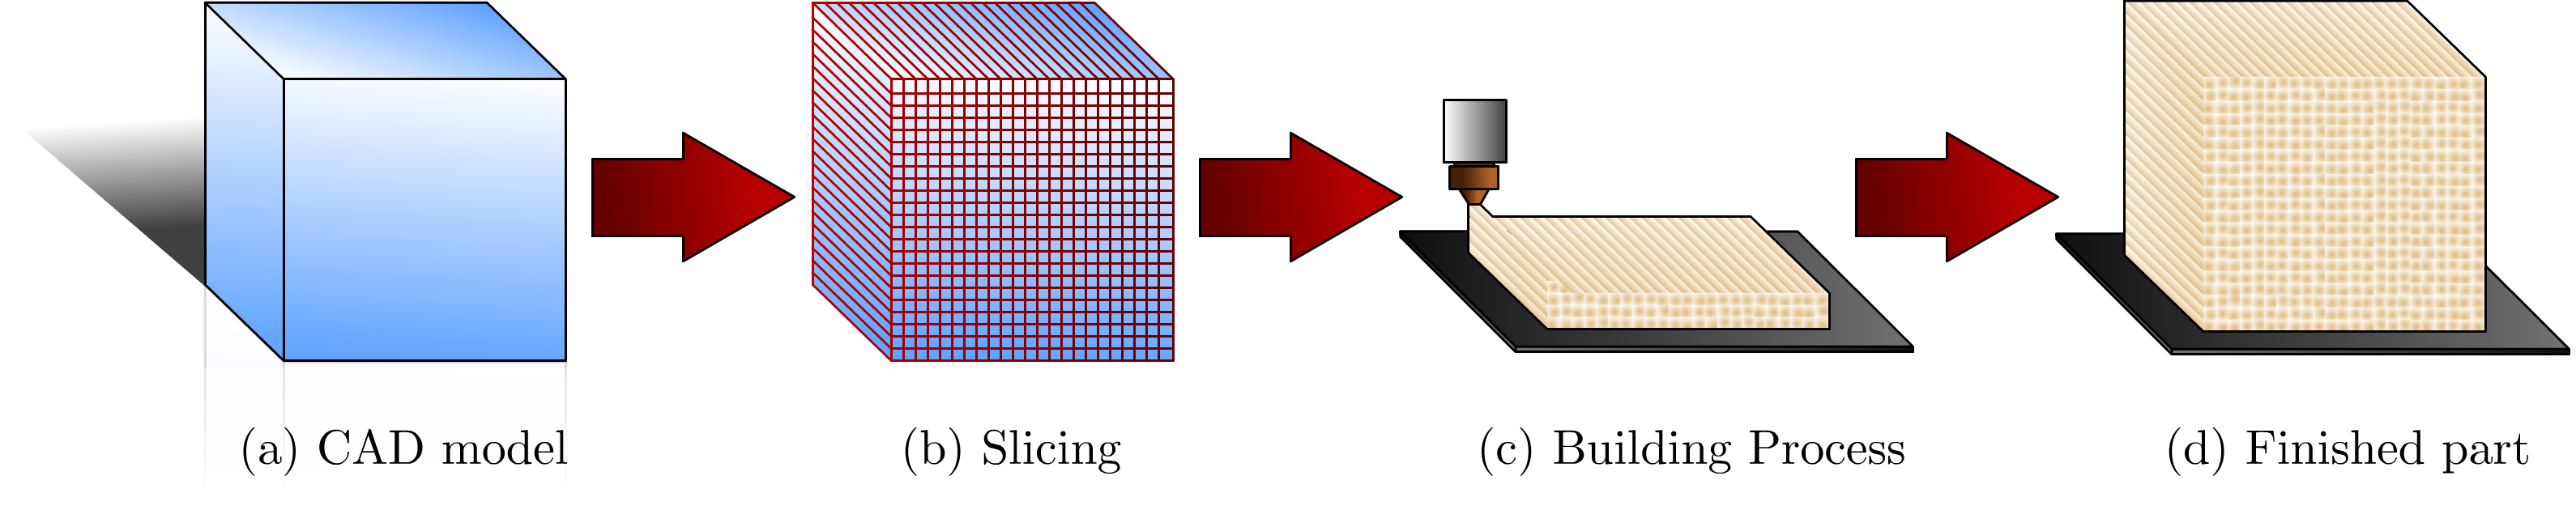
\includegraphics[width=\linewidth]{AM_flowchart_1}
	\caption{Process flow of AM} \label{fig:AM_flow}
\end{figure}

While all AM technologies operate on the same basic process flow described above, the specifics of each AM technique vary substantially, ranging from processes that use paper and binder, all the way through metal-based, laser tracing technologies. Since this is a rapidly evolving field, no general consensus exists for classifying the multiple AM processes available. However, the classification system proposed under the ASTM/ISO 52900 standard \cite{ASTM52900}, has been somewhat accepted by the field and divides AM technologies as follows:
\begin{enumerate}
	\item \textbf{Binder Jetting}: AM techniques where a binding agent is used to selectively promote cohesion in powder materials -generally gypsum, sand or metallic powders \cite{3DHubs2018}.
	\item \textbf{Directed Energy Deposition}: AM processes where a focused thermal energy source (i.e. laser, electron beam, plasma arc) is used to fuse materials as they are being deposited in the build volume. Materials are almost exclusively metals \cite{ASTM52900,3DHubs2018}.
	\item \textbf{Material Extrusion}: In this type of AM technology, material is dispensed through a nozzle or orifice. Fused Filament Fabrication belongs to this classification. Materials are almost exclusively thermoplastics \cite{ASTM52900,3DHubs2018}.
	\item \textbf{Material Jetting}: AM techniques where build material is deposited selectively in droplets. Materials are usually wax or thermoplastics, but there are examples of metal-based, material jetting techniques \cite{ASTM52900,3DHubs2018}.
	\item \textbf{Powder Bed Fusion}: AM processes where portions of a powder bed are selectively fused through application of thermal energy. \emph{Selective Laser Sintering} (SLS) belongs to this category. Materials are usually thermoplastic polymers or metals \cite{ASTM52900,3DHubs2018}. 
	\item \textbf{Sheet Lamination}: In this type of AM technology, the final part is formed by bonding sheets of material -usually paper or composites \cite{ASTM52900,3DHubs2018}. 
	\item \textbf{Vat Photopolymerization}: In this AM process, a liquid photopolymer is selectively cured by a light source. \emph{Stereolithography} (SLA), arguably the first AM technology, belongs to this category. Due to the nature of this technique, the only materials used are photopolymers \cite{ASTM52900,3DHubs2018}.
\end{enumerate} 

\subsection{Advantages and Disadvantages}\label{subsec:AMAdDis} 
Since AM processes allow a relatively direct conversion of a CAD model into a constructed object, they were originally exclusively used for prototype development. For this reason, they were initially classified as \textquotedblleft \emph{Rapid Prototyping}\textquotedblright~(RP) technologies. This terminology is still used today, however, it is being superseded by \emph{Additive Manufacturing} since the potential to become a proper fabrication technique exists \cite{Gibson2015}. However, while being capable of quickly jumping from part design to manufacturing is a great advantage, AM has its own set of drawbacks. Table \ref{tab:AM_AdDis} summarizes the most noteworthy set of advantages and disadvantages typical of most AM technologies.

\begin{table}[h]
	\centering
	\caption{Advantages and Disadvantages of Additive Manufacturing}
	\label{tab:AM_AdDis}
	\begin{tabular}{ll}
		\hline
		Advantages & Disadvantages \\ \hline
		&               \\
		&               \\
		&               \\ \hline
	\end{tabular}
\end{table}   
\section{Fused Filament Fabrication}

%Nomenclature introduced in this chapter:
\nomenclature[A]{SLA}{Stereolithography}% 
\nomenclature[A]{SLS}{Selective Laser Sintering}%
\end{document}